 \setlength{\tabcolsep}{1pt}

  \begin{figure*}[h]
    \footnotesize
    \small
    \centering
    \begin{tabular}{ccccccc}
      \hline

      \multirow{2}{*}{Input} &  (i) & (ii) & (iii) & (iv) & (v) & (vi) \\
      &  CA guidance &  $\vz_t$  guidance & SA replace.&  SA guidance &   (iv)+CA replace. &  (v) + LB \\
      \hline
      \multicolumn{7}{c}{``\textit{a girl with blonde hair \textcolor{RoyalBlue}{\textbf{and a fluffy rainbow hat}} smiling}"} \\
      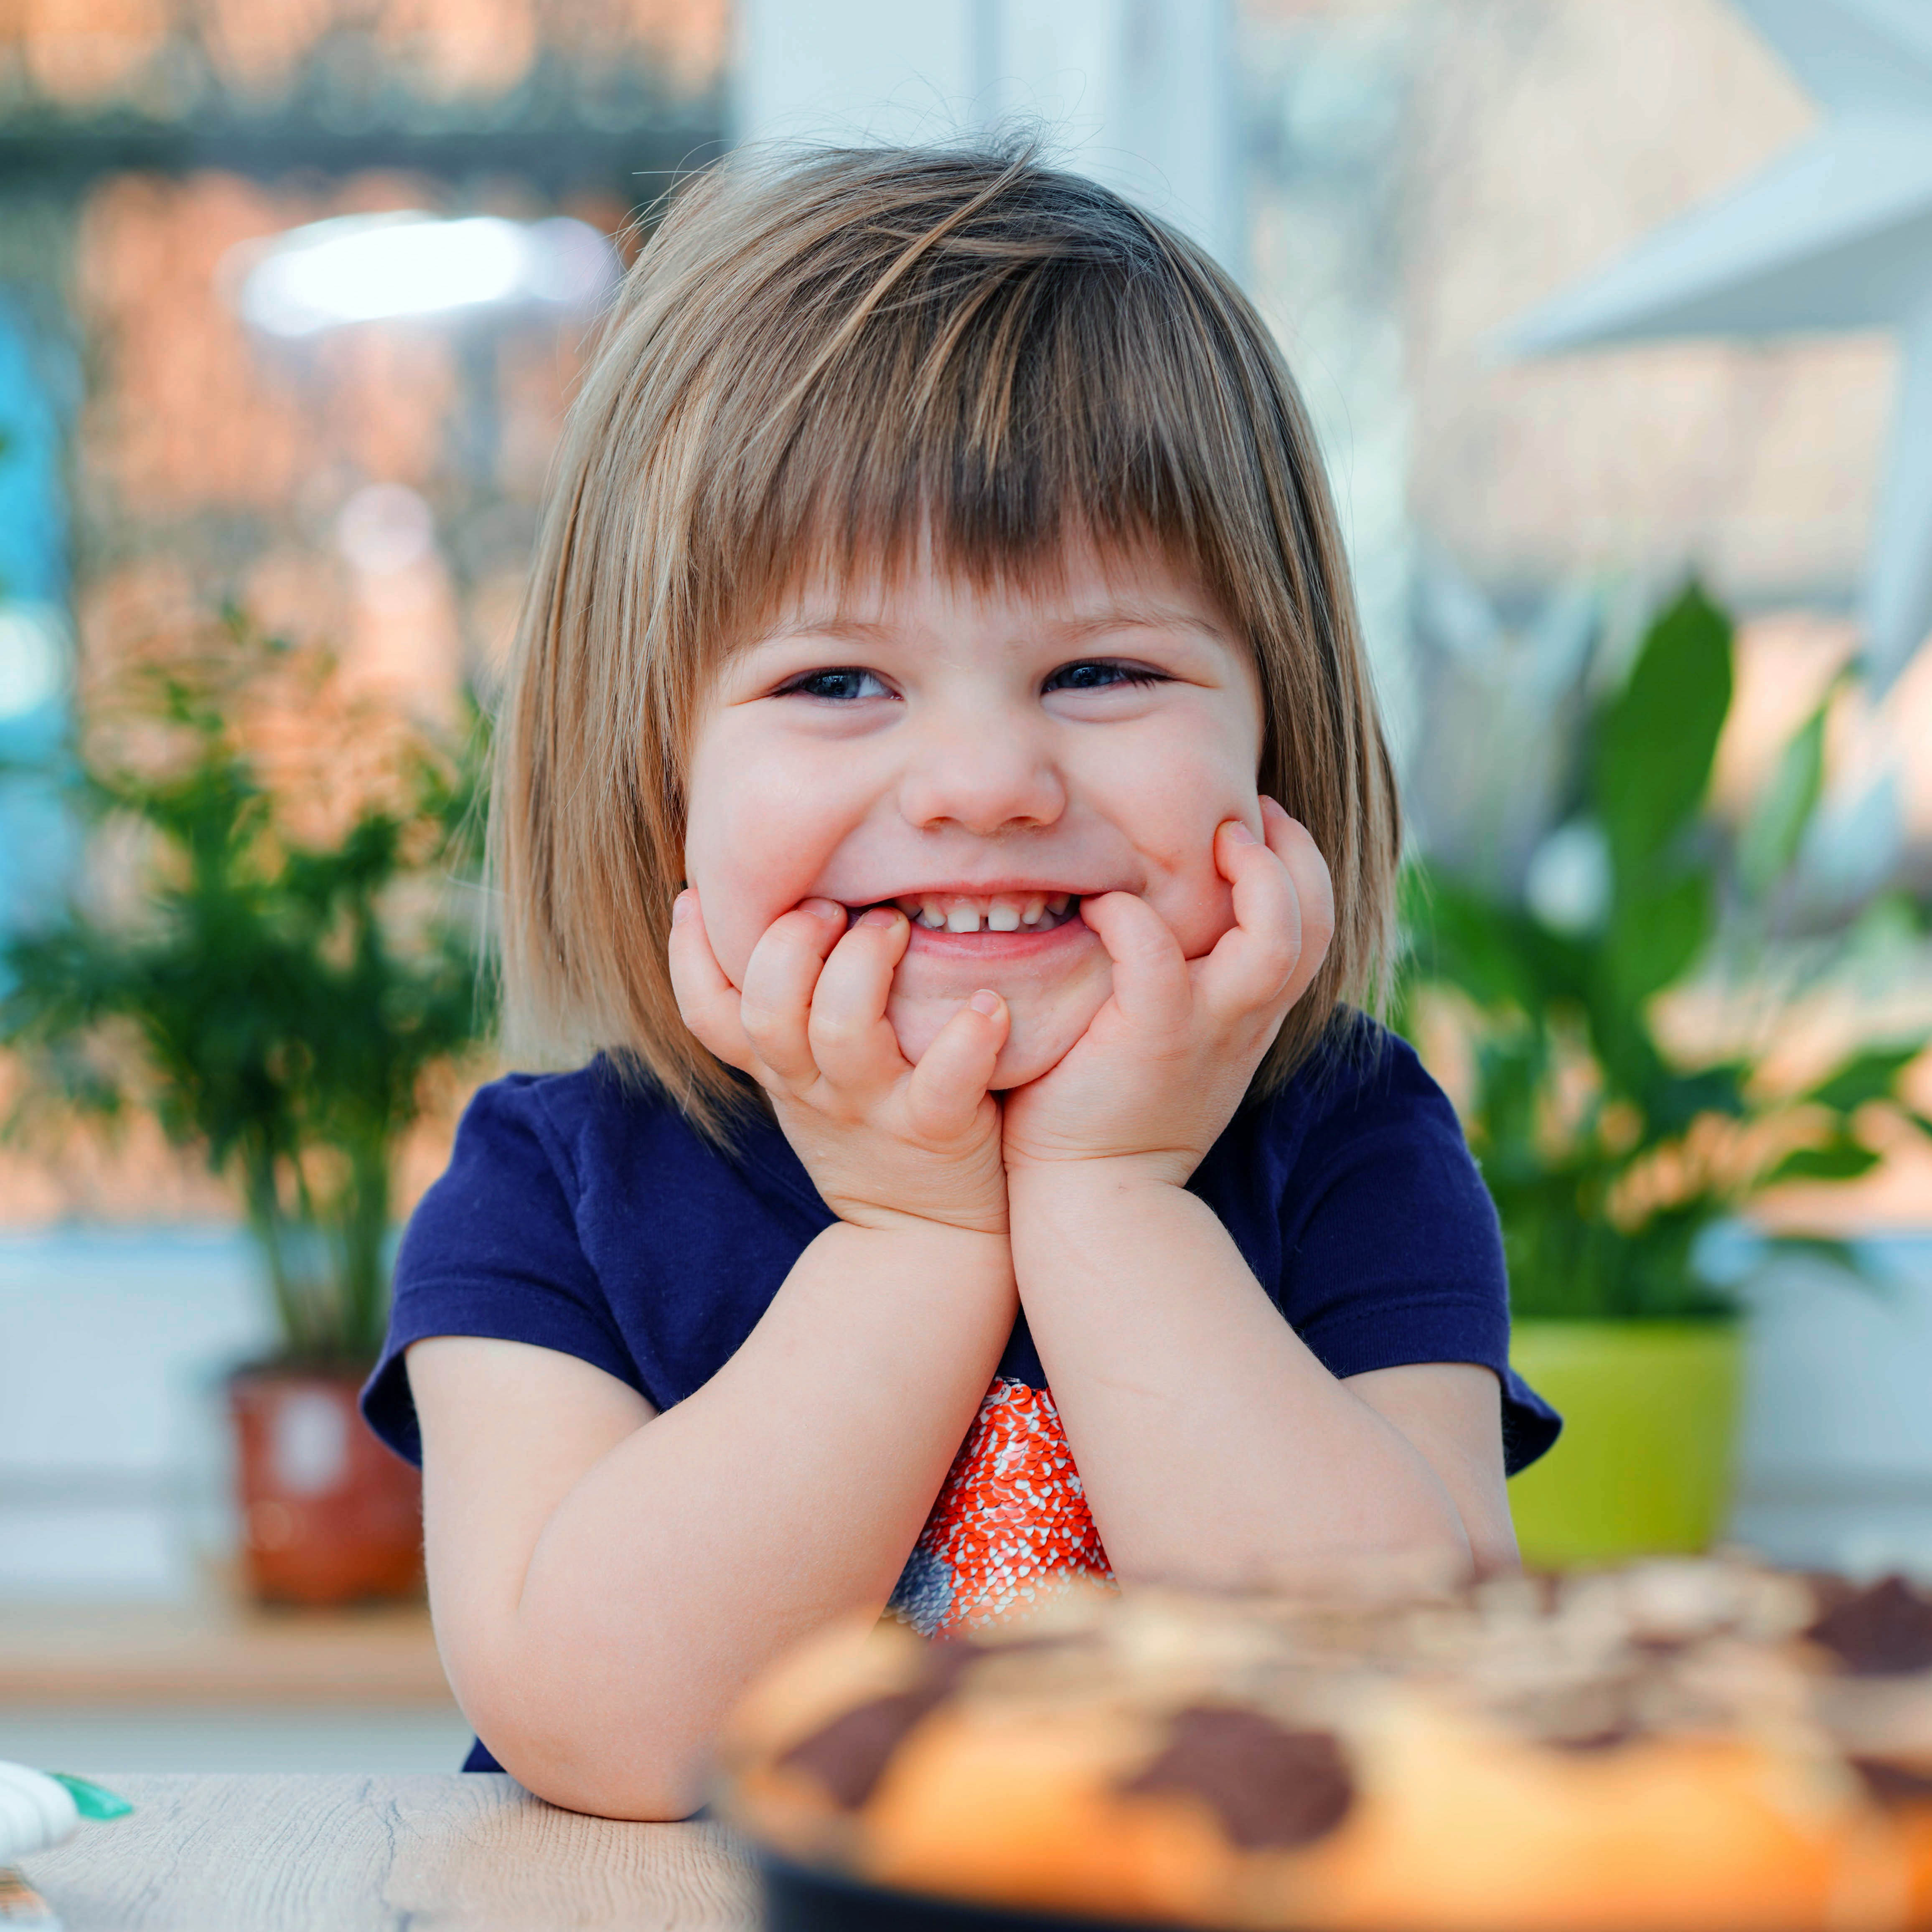
\includegraphics[width=2.1cm, height=2.1cm]{fig/ablation/1_ablation_input} & 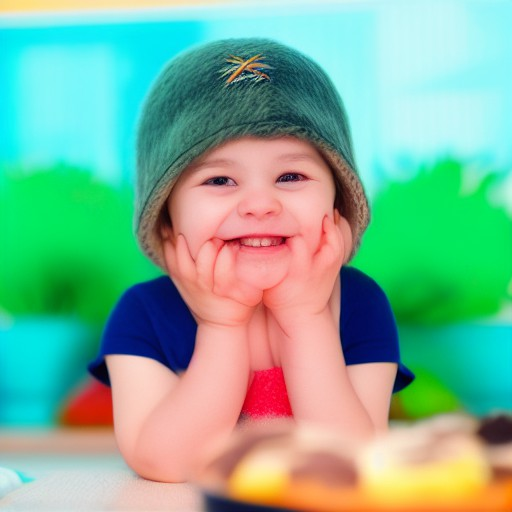
\includegraphics[width=2.1cm, height=2.1cm]{fig/ablation/1_ablation_2} &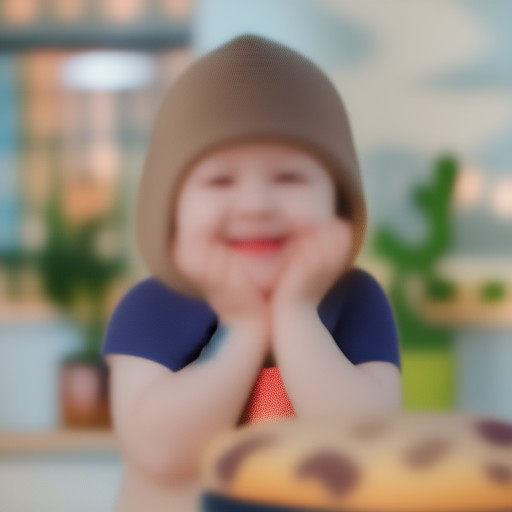
\includegraphics[width=2.1cm, height=2.1cm]{fig/ablation/1_ablation_3} &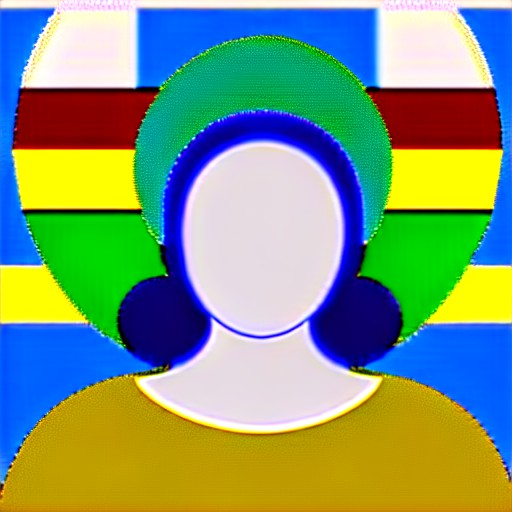
\includegraphics[width=2.1cm, height=2.1cm]{fig/ablation/1_ablation_4_cfg75} &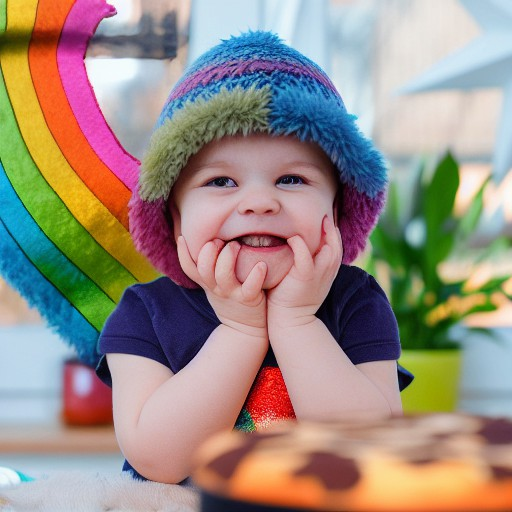
\includegraphics[width=2.1cm, height=2.1cm]{fig/ablation/1_ablation_1} &
\includegraphics[width=2.1cm, height=2.1cm]{fig/ablation/1_ablation_5} &
\includegraphics[width=2.1cm, height=2.1cm]{fig/ablation/1_ablation_6} \\
      \multicolumn{7}{c}{``\textit{a baby with a stuffed \textcolor{BrickRed}{\st{monkey}} \textcolor{RoyalBlue}{\textbf{zebra}} in a car}"} \\
      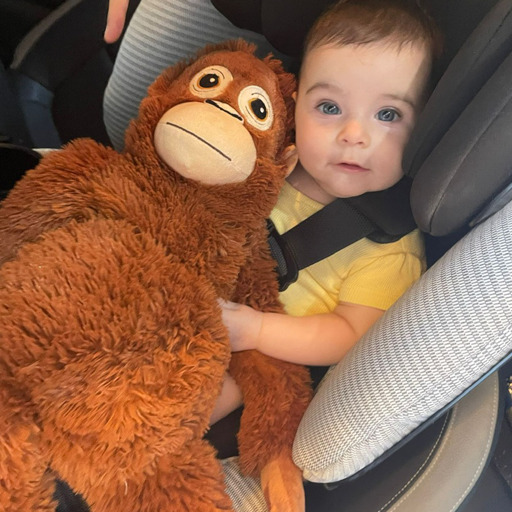
\includegraphics[width=2.1cm, height=2.1cm]{fig/ablation/0_ablation_input} & 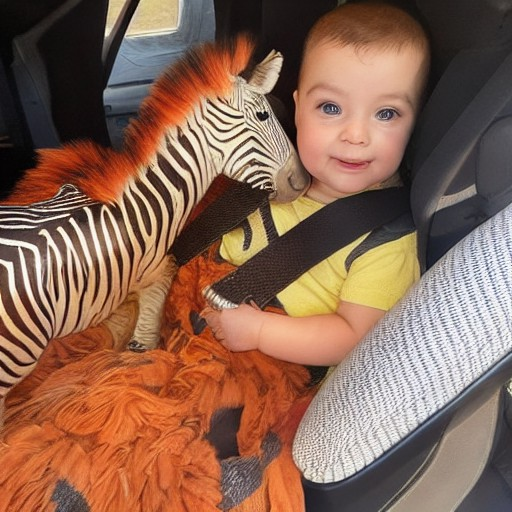
\includegraphics[width=2.1cm, height=2.1cm]{fig/ablation/0_ablation_2} &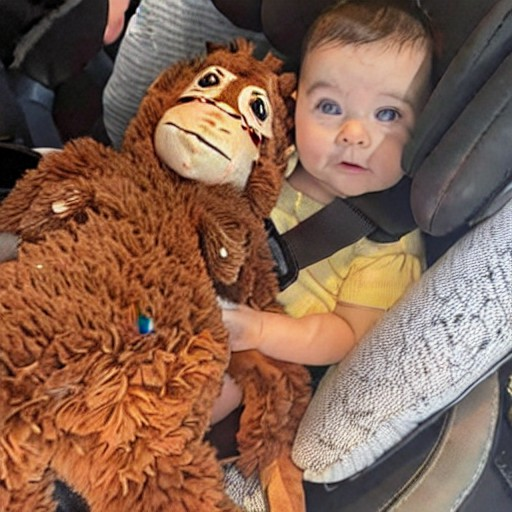
\includegraphics[width=2.1cm, height=2.1cm]{fig/ablation/0_ablation_3} &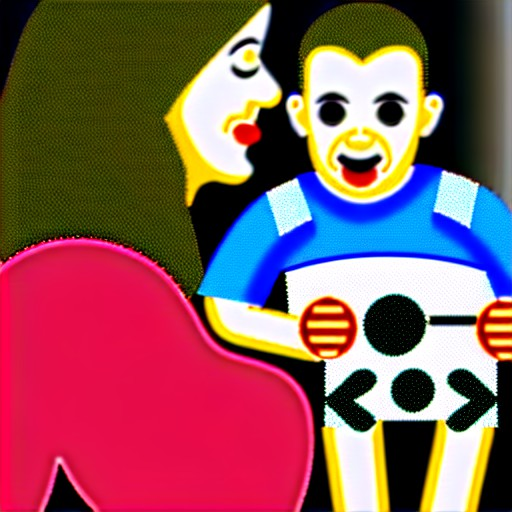
\includegraphics[width=2.1cm, height=2.1cm]{fig/ablation/0_ablation_4}
      &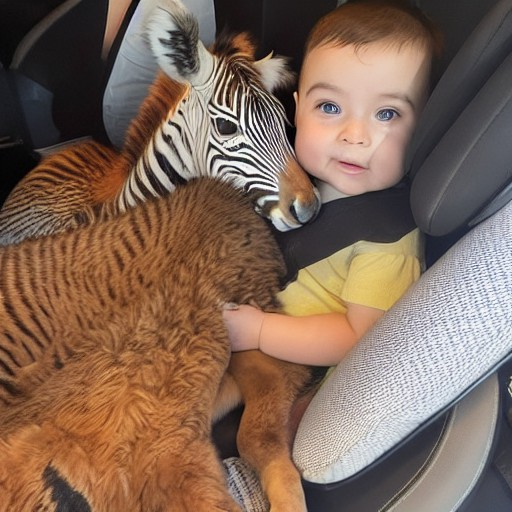
\includegraphics[width=2.1cm, height=2.1cm]{fig/ablation/0_ablation_1} &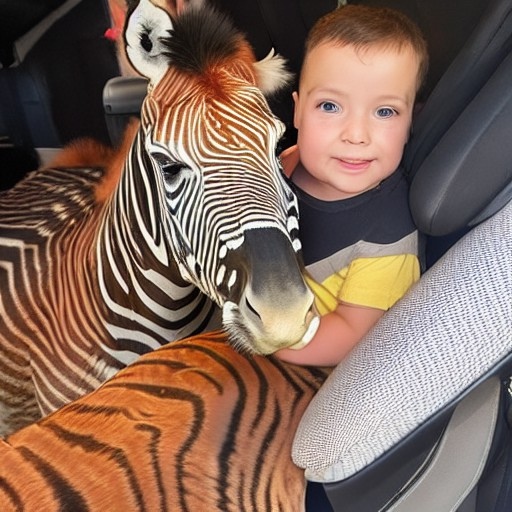
\includegraphics[width=2.1cm, height=2.1cm]{fig/ablation/0_ablation_5} &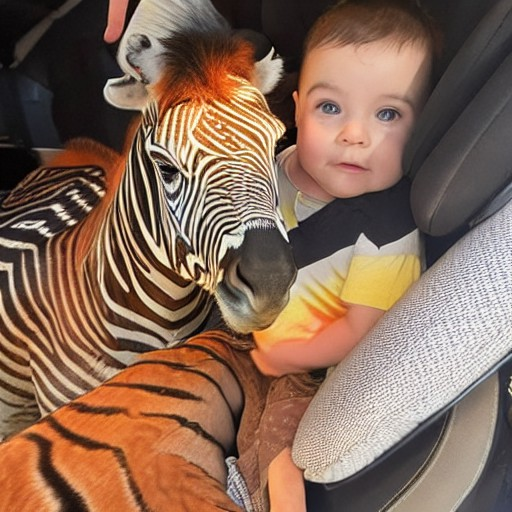
\includegraphics[width=2.1cm, height=2.1cm]{fig/ablation/0_ablation_6} \\
      \hline
      % ... Add more rows as needed
    \end{tabular}
    \caption{{\modified{}Qualitative results of the} ablation study. Each column corresponds to a configuration described in Table \ref{tab:ablation_piebench}.}
    \label{fig:ablationquali}
  \end{figure*}